\documentclass[tikz,border=5pt]{standalone}
\usepackage{lmodern}
\definecolor{figureblue}{HTML}{1455C0}
\begin{document}
\pagecolor{white}
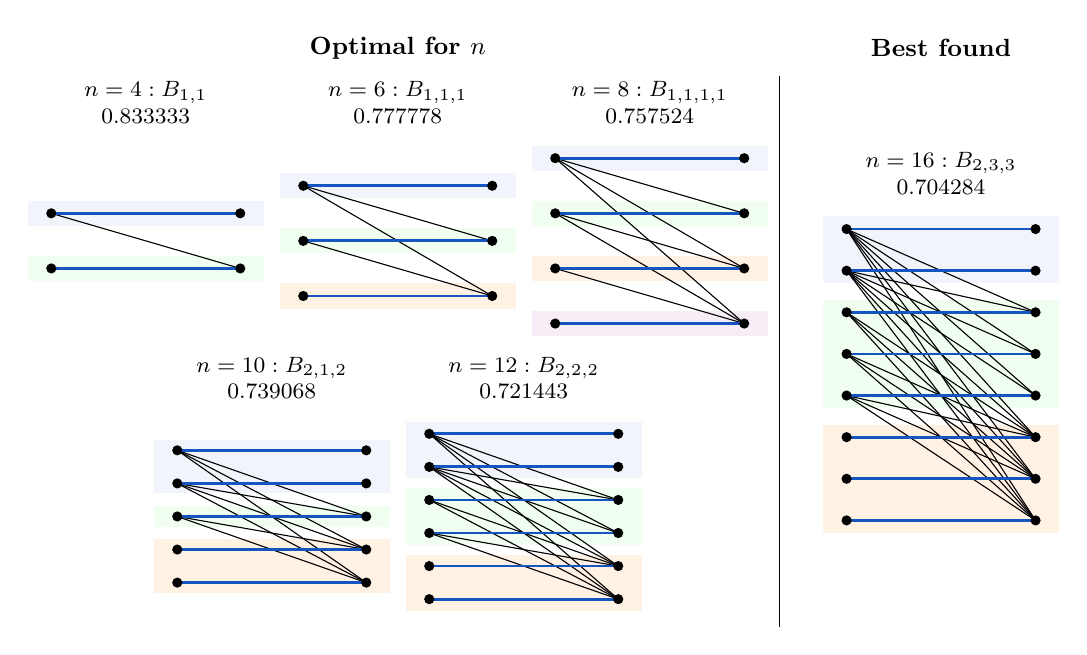
\begin{tikzpicture}[x=1cm,y=1cm,
 vertex/.style={circle,fill=black,inner sep=1.3pt},
 cross/.style={black,line width=.4pt},
 matching/.style={figureblue,line width=1pt},
 every node/.style={font=\footnotesize}]
\node[font=\small\bfseries] at (4.4,1.4) {Optimal for $n$};
\node[font=\small\bfseries] at (11.3,1.4) {Best found};
\draw[black,line width=.4pt] (9.25,1.05)--(9.25,-5.95);
\begin{scope}[shift={(0,0)}]
\node[align=center,anchor=south] at (1.2,.32) {$n=4: B_{1,1}$\\$0.833333$};
\fill[figureblue!6] (-.30,-0.5400) rectangle (2.70,-0.8600);
\fill[green!6] (-.30,-1.2400) rectangle (2.70,-1.5600);
\draw[cross] (0,-0.7000)--(2.4,-1.4000);
\draw[matching] (0,-0.7000)--(2.4,-0.7000);
\node[vertex] at (0,-0.7000) {}; \node[vertex] at (2.4,-0.7000) {};
\draw[matching] (0,-1.4000)--(2.4,-1.4000);
\node[vertex] at (0,-1.4000) {}; \node[vertex] at (2.4,-1.4000) {};
\end{scope}
\begin{scope}[shift={(3.2,0)}]
\node[align=center,anchor=south] at (1.2,.32) {$n=6: B_{1,1,1}$\\$0.777778$};
\fill[figureblue!6] (-.30,-0.1900) rectangle (2.70,-0.5100);
\fill[green!6] (-.30,-0.8900) rectangle (2.70,-1.2100);
\fill[orange!10] (-.30,-1.5900) rectangle (2.70,-1.9100);
\draw[cross] (0,-0.3500)--(2.4,-1.0500);
\draw[cross] (0,-0.3500)--(2.4,-1.7500);
\draw[cross] (0,-1.0500)--(2.4,-1.7500);
\draw[matching] (0,-0.3500)--(2.4,-0.3500);
\node[vertex] at (0,-0.3500) {}; \node[vertex] at (2.4,-0.3500) {};
\draw[matching] (0,-1.0500)--(2.4,-1.0500);
\node[vertex] at (0,-1.0500) {}; \node[vertex] at (2.4,-1.0500) {};
\draw[matching] (0,-1.7500)--(2.4,-1.7500);
\node[vertex] at (0,-1.7500) {}; \node[vertex] at (2.4,-1.7500) {};
\end{scope}
\begin{scope}[shift={(6.4,0)}]
\node[align=center,anchor=south] at (1.2,.32) {$n=8: B_{1,1,1,1}$\\$0.757524$};
\fill[figureblue!6] (-.30,0.1600) rectangle (2.70,-0.1600);
\fill[green!6] (-.30,-0.5400) rectangle (2.70,-0.8600);
\fill[orange!10] (-.30,-1.2400) rectangle (2.70,-1.5600);
\fill[violet!7] (-.30,-1.9400) rectangle (2.70,-2.2600);
\draw[cross] (0,0.0000)--(2.4,-0.7000);
\draw[cross] (0,0.0000)--(2.4,-1.4000);
\draw[cross] (0,0.0000)--(2.4,-2.1000);
\draw[cross] (0,-0.7000)--(2.4,-1.4000);
\draw[cross] (0,-0.7000)--(2.4,-2.1000);
\draw[cross] (0,-1.4000)--(2.4,-2.1000);
\draw[matching] (0,0.0000)--(2.4,0.0000);
\node[vertex] at (0,0.0000) {}; \node[vertex] at (2.4,0.0000) {};
\draw[matching] (0,-0.7000)--(2.4,-0.7000);
\node[vertex] at (0,-0.7000) {}; \node[vertex] at (2.4,-0.7000) {};
\draw[matching] (0,-1.4000)--(2.4,-1.4000);
\node[vertex] at (0,-1.4000) {}; \node[vertex] at (2.4,-1.4000) {};
\draw[matching] (0,-2.1000)--(2.4,-2.1000);
\node[vertex] at (0,-2.1000) {}; \node[vertex] at (2.4,-2.1000) {};
\end{scope}
\begin{scope}[shift={(1.6,-3.5)}]
\node[align=center,anchor=south] at (1.2,.32) {$n=10: B_{2,1,2}$\\$0.739068$};
\fill[figureblue!6] (-.30,-0.0820) rectangle (2.70,-0.7580);
\fill[green!6] (-.30,-0.9220) rectangle (2.70,-1.1780);
\fill[orange!10] (-.30,-1.3420) rectangle (2.70,-2.0180);
\draw[cross] (0,-0.2100)--(2.4,-1.0500);
\draw[cross] (0,-0.2100)--(2.4,-1.4700);
\draw[cross] (0,-0.2100)--(2.4,-1.8900);
\draw[cross] (0,-0.6300)--(2.4,-1.0500);
\draw[cross] (0,-0.6300)--(2.4,-1.4700);
\draw[cross] (0,-0.6300)--(2.4,-1.8900);
\draw[cross] (0,-1.0500)--(2.4,-1.4700);
\draw[cross] (0,-1.0500)--(2.4,-1.8900);
\draw[matching] (0,-0.2100)--(2.4,-0.2100);
\node[vertex] at (0,-0.2100) {}; \node[vertex] at (2.4,-0.2100) {};
\draw[matching] (0,-0.6300)--(2.4,-0.6300);
\node[vertex] at (0,-0.6300) {}; \node[vertex] at (2.4,-0.6300) {};
\draw[matching] (0,-1.0500)--(2.4,-1.0500);
\node[vertex] at (0,-1.0500) {}; \node[vertex] at (2.4,-1.0500) {};
\draw[matching] (0,-1.4700)--(2.4,-1.4700);
\node[vertex] at (0,-1.4700) {}; \node[vertex] at (2.4,-1.4700) {};
\draw[matching] (0,-1.8900)--(2.4,-1.8900);
\node[vertex] at (0,-1.8900) {}; \node[vertex] at (2.4,-1.8900) {};
\end{scope}
\begin{scope}[shift={(4.8,-3.5)}]
\node[align=center,anchor=south] at (1.2,.32) {$n=12: B_{2,2,2}$\\$0.721443$};
\fill[figureblue!6] (-.30,0.1470) rectangle (2.70,-0.5670);
\fill[green!6] (-.30,-0.6930) rectangle (2.70,-1.4070);
\fill[orange!10] (-.30,-1.5330) rectangle (2.70,-2.2470);
\draw[cross] (0,0.0000)--(2.4,-0.8400);
\draw[cross] (0,0.0000)--(2.4,-1.2600);
\draw[cross] (0,0.0000)--(2.4,-1.6800);
\draw[cross] (0,0.0000)--(2.4,-2.1000);
\draw[cross] (0,-0.4200)--(2.4,-0.8400);
\draw[cross] (0,-0.4200)--(2.4,-1.2600);
\draw[cross] (0,-0.4200)--(2.4,-1.6800);
\draw[cross] (0,-0.4200)--(2.4,-2.1000);
\draw[cross] (0,-0.8400)--(2.4,-1.6800);
\draw[cross] (0,-0.8400)--(2.4,-2.1000);
\draw[cross] (0,-1.2600)--(2.4,-1.6800);
\draw[cross] (0,-1.2600)--(2.4,-2.1000);
\draw[matching] (0,0.0000)--(2.4,0.0000);
\node[vertex] at (0,0.0000) {}; \node[vertex] at (2.4,0.0000) {};
\draw[matching] (0,-0.4200)--(2.4,-0.4200);
\node[vertex] at (0,-0.4200) {}; \node[vertex] at (2.4,-0.4200) {};
\draw[matching] (0,-0.8400)--(2.4,-0.8400);
\node[vertex] at (0,-0.8400) {}; \node[vertex] at (2.4,-0.8400) {};
\draw[matching] (0,-1.2600)--(2.4,-1.2600);
\node[vertex] at (0,-1.2600) {}; \node[vertex] at (2.4,-1.2600) {};
\draw[matching] (0,-1.6800)--(2.4,-1.6800);
\node[vertex] at (0,-1.6800) {}; \node[vertex] at (2.4,-1.6800) {};
\draw[matching] (0,-2.1000)--(2.4,-2.1000);
\node[vertex] at (0,-2.1000) {}; \node[vertex] at (2.4,-2.1000) {};
\end{scope}
\begin{scope}[shift={(10.1,-0.9)}]
\node[align=center,anchor=south] at (1.2,.32) {$n=16: B_{2,3,3}$\\$0.704284$};
\fill[figureblue!6] (-.30,0.1600) rectangle (2.70,-0.6886);
\fill[green!6] (-.30,-0.8971) rectangle (2.70,-2.2743);
\fill[orange!10] (-.30,-2.4829) rectangle (2.70,-3.8600);
\draw[cross] (0,0.0000)--(2.4,-1.0571);
\draw[cross] (0,0.0000)--(2.4,-1.5857);
\draw[cross] (0,0.0000)--(2.4,-2.1143);
\draw[cross] (0,0.0000)--(2.4,-2.6429);
\draw[cross] (0,0.0000)--(2.4,-3.1714);
\draw[cross] (0,0.0000)--(2.4,-3.7000);
\draw[cross] (0,-0.5286)--(2.4,-1.0571);
\draw[cross] (0,-0.5286)--(2.4,-1.5857);
\draw[cross] (0,-0.5286)--(2.4,-2.1143);
\draw[cross] (0,-0.5286)--(2.4,-2.6429);
\draw[cross] (0,-0.5286)--(2.4,-3.1714);
\draw[cross] (0,-0.5286)--(2.4,-3.7000);
\draw[cross] (0,-1.0571)--(2.4,-2.6429);
\draw[cross] (0,-1.0571)--(2.4,-3.1714);
\draw[cross] (0,-1.0571)--(2.4,-3.7000);
\draw[cross] (0,-1.5857)--(2.4,-2.6429);
\draw[cross] (0,-1.5857)--(2.4,-3.1714);
\draw[cross] (0,-1.5857)--(2.4,-3.7000);
\draw[cross] (0,-2.1143)--(2.4,-2.6429);
\draw[cross] (0,-2.1143)--(2.4,-3.1714);
\draw[cross] (0,-2.1143)--(2.4,-3.7000);
\draw[matching] (0,0.0000)--(2.4,0.0000);
\node[vertex] at (0,0.0000) {}; \node[vertex] at (2.4,0.0000) {};
\draw[matching] (0,-0.5286)--(2.4,-0.5286);
\node[vertex] at (0,-0.5286) {}; \node[vertex] at (2.4,-0.5286) {};
\draw[matching] (0,-1.0571)--(2.4,-1.0571);
\node[vertex] at (0,-1.0571) {}; \node[vertex] at (2.4,-1.0571) {};
\draw[matching] (0,-1.5857)--(2.4,-1.5857);
\node[vertex] at (0,-1.5857) {}; \node[vertex] at (2.4,-1.5857) {};
\draw[matching] (0,-2.1143)--(2.4,-2.1143);
\node[vertex] at (0,-2.1143) {}; \node[vertex] at (2.4,-2.1143) {};
\draw[matching] (0,-2.6429)--(2.4,-2.6429);
\node[vertex] at (0,-2.6429) {}; \node[vertex] at (2.4,-2.6429) {};
\draw[matching] (0,-3.1714)--(2.4,-3.1714);
\node[vertex] at (0,-3.1714) {}; \node[vertex] at (2.4,-3.1714) {};
\draw[matching] (0,-3.7000)--(2.4,-3.7000);
\node[vertex] at (0,-3.7000) {}; \node[vertex] at (2.4,-3.7000) {};
\end{scope}
\end{tikzpicture}
\end{document}
